\documentclass[draft,12pt,headsepline,footsepline,paper=letter]{scrreprt}
\pagestyle{headings}

\usepackage[utf8]{inputenc}
\usepackage[T1]{fontenc}
\def\spanishoptions{es-noquoting,es-nolists,mexico-com}
\usepackage[spanish]{babel}

\usepackage{makeidx}
\makeindex

\usepackage[nonumberlist]{glossaries}
\makeglossaries

\usepackage[final]{graphicx}
\DeclareGraphicsExtensions{.pdf,.png,.jpg}
\graphicspath{{media/}}

\iftrue % outline for images
\usepackage{scrhack}
\usepackage{float}
\floatstyle{boxed}
\restylefloat{figure}
\fi

\usepackage{natbib}
\usepackage{amsmath,amssymb, bm}
\usepackage{enumerate}
\usepackage{ragged2e}

\usepackage{setspace}
\onehalfspacing
\frenchspacing
\recalctypearea

\usepackage{pdfsync}

\begin{document}

\title{Planificación de horarios educacionales}
\author{Héctor Arciga}
\date{\today}

\maketitle

\begin{spacing}{1}
\tableofcontents
\glsaddall 
\printglossaries
\listoffigures
\listoftables
\end{spacing}

% Contenido

\chapter{Introducción}

% Capítulo: Introducción

\section{Antecedentes y motivación}

Las instituciones educativas como factor de cambio social juegan un papel importante en el amoldamiento del individuo, en particular cuando la formación es obligatoria y a modo del Estado. Es bajo estas condiciones que el gestor escolar debe diseñar sus estrategias para alcanzar sus objetivos institucionales. 
Si bien el gestor escolar en el sector público no cuenta con el mismo grado de laxitud operativa que su contra-parte en la iniciativa privada, ambos tienen alternativas de acción similares para afectar el desempeño de su institución.
Mucho se ha hablado de maneras para mejorar el nivel educativo en las instituciones educativas desde la inversión de recursos en infraestructura; la capacitación continua de los docentes; el aprovisionamiento gratuito de útiles escolares, uniformes, alimentos; la  inclusión de las nuevas tecnologías informáticas en la pedagogía; mejoras en las condiciones laborales del magisterio; 


\section{Objetivos de la investigación}

\index{gestor escolar}\index{métricas de desempeño}\index{formulación matemática}
Esta tesis investiga la problemática de la elaboración de horarios en instituciones docentes y el impacto potencial de su formulación en distintas métricas de desempeño educacional relevantes para el gestor escolar. 
El fin primordial del trabajo es investigar de qué manera puede el gestor escolar hacer uso de estas técnicas, para la consecución de sus estrategias.
Para poder cumplir con esta finalidad, los siguientes objetivos son considerados:
\begin{enumerate}[1]
\item La investigación de las distintas problemáticas en la planificación de horarios en instituciones docentes.
\item Las distintas formulaciones matemáticas de los problemas de planificación de horarios.
\item Los algoritmos de solución disponibles para este tipo de modelos matemáticos.
\item Los antecedentes históricos de técnicas de optimación aplicados a partir del surgimiento de los ordenadores.
\item La recopilación de las métricas de desempeño educacional relevantes para los gestores escolares.
\item Una investigación de las limitantes más comunes utilizadas en las formulaciones de los problemas de planificación de horarios.
\end{enumerate}

\section{Descripción de la tesis}

Esta tesis consiste de ocho capítulos. El presente capítulo presenta los antecedentes, motivación y objetivos de la investigación. El resto de la tesis está organizada de la siguiente manera:

El Capítulo 2 presenta una visión general de la problemática así como su clasificación en la literatura.

Los preliminares de la calendarización en general aparecen en el Capítulo 3.

En el Capítulo 4 se detallan los modelos matemáticos y los algoritmos existentes para su solución así como una propuesta de un lenguaje en común para la representación de los problemas.

Las limitantes y funciones objetivo más comunes en la literatura se exponen en el Capítulo 5.

El papel del gestor escolar se discute en el Capítulo 6.

En el Capítulo 7 se hace una exposición del tipo de herramientas existentes para la solución de estos problemas así como un listado de algunas opciones de software encontradas.

Por último, en el Capítulo 8 se presenta un resumen del trabajo de investigación, las contribuciones hechas en el mismo, el trabajo futuro y la diseminación de trabajo.

\chapter{Una visión general del problema}

% Capítulo: Una visión general del problema

\section{Introducción}

\index{horarios!planificación}
En este capítulo se hace una revisión bibliográfica poniéndo énfasis en los aspectos fundamentales del área de investigación. Se introduce la definición del problema general de planificación de horarios así como los términos relevantes al ámbito de estudio. 

, en específico la problemática relevante a las instituciones docentes así como las limitantes que tales problemas deben considerar \citep[p.~8]{abdullah06heuristic-approaches}. Se precisan los términos utilizados en el ámbito

El capítulo comprende 


\section{¿Qué es la planificación de horarios?}

\index{horarios!planificación!problema general}
\citet[p.~53]{wren95scheduling-timetabling} definió la planificación de horarios como “la asignación, sujeta a limitantes\index{limitantes}, de recursos a objetos dados siendo puestos en espacio-tiempo, de tal manera que se satisfagan tanto como sea posible un conjunto de objetivos deseados.”

\subsection{Definiciones de términos}

Es necesario aclarar algunos términos prevalentes en este trabajo pues en la literatura relevante son utilizados de manera muy distinta. Siguiendo la pauta de \citet[p.~46]{wren95scheduling-timetabling} el trabajo comienza con el más ampliamente utilizado: programación\index{programación} (\textit{scheduling}). ¿Qué es la programación?

La programación es una palabra común —forma parte del vocabulario del día a día— aunque no siempre se tenga una idea clara de su significado. En realidad, no la acción de programar lo que es un concepto común en la vida diaria, son más bien los horarios. Un horario es un plan o documento tangible, tal como el horario de salidas de un autobus o un horario de clases. Un horario señala cuándo debe suceder algún evento; especifíca un plan para el tiempo de ocurrencia de ciertas actividades y contesta la pregunta, “Si todo va bien, ¿cuándo ocurrirá un evento en particular?” 
Digamos que es deseable saber cuándo la cena será servida o cuándo un autobus saldrá a su destino. En estos casos, el evento de interés es la compleción de una actividad en particular —como lo es la preparación de la cena— o el comienzo de una actividad en particular —como el viaje en autobus—.
Las respuestas a la pregunta “¿cuándo?” usualmente están ligadas con información acerca del tiempo. La cena está programada para ser servida a las 18:00, el autobus está programado para salir a las 8:00. Sin embargo, una respuesta igualmente útil puede ser dada en términos de secuencia en lugar de tiempo: es decir, la cena será servida tan pronto como el platillo principal esté horneado, o el autobus partirá a su destino en cuanto su limpieza y mantenimiento sean completados. Por lo tanto, la pregunta “¿cuándo?” puede ser respondida ya sea con información de tiempo o de secuencia obtenida a partir de un horario \citep[p.~1]{Baker2009}.

De manera intuitiva, se puede pensar que la programación es el acto de producir un horario, sin embargo rara vez se consideran los detalles del proceso que ello conlleva. De hecho, aunque se piense en un horario como algo tangible, el proceso de la programación parece no serlo, hasta que es considerado con cierto detenimiento. El problema es comúnmente atacado en dos pasos: secuenciación y programación. En el primer paso, se planifica una secuencia o se decide cómo elegir la siguiente tarea. En el segundo paso, se planifica la hora de inicio, y tal vez la hora de terminación, de cada tarea \citep[p.~2]{Baker2009}. 


\section{Clasificación de los problemas}

\index{clasificación}
El problema de la planificación de horarios educacionales\index{horarios!educacionales} se clasifica en tres clases principalmente:
horarios de clases\index{horarios!de clases} (\textit{school timetabling}),
calendarización de cursos\index{calendarización!de cursos} (\textit{course timetabling}) y
calendarización de exámenes\index{calendarización!de exámenes} (\textit{examination timetabling}) \citep[p.~88]{schaerf99a-survey-of-automated}.

Todos tienen en común las características básicas del problema general de planificación de horarios\index{horarios!problema general} pero pueden presentar diferencias significativas entre ellos. Cada problema cuenta con su propias limitantes, requerimientos y reglas. Son agrupados por su ámbito de aplicación en horarios en escuelas\index{horarios!en escuelas} y horarios en universidades\index{horarios!en universidades} \citep[p.~10]{abdullah06heuristic-approaches}.

\begin{figure}[hbtp]
\centering
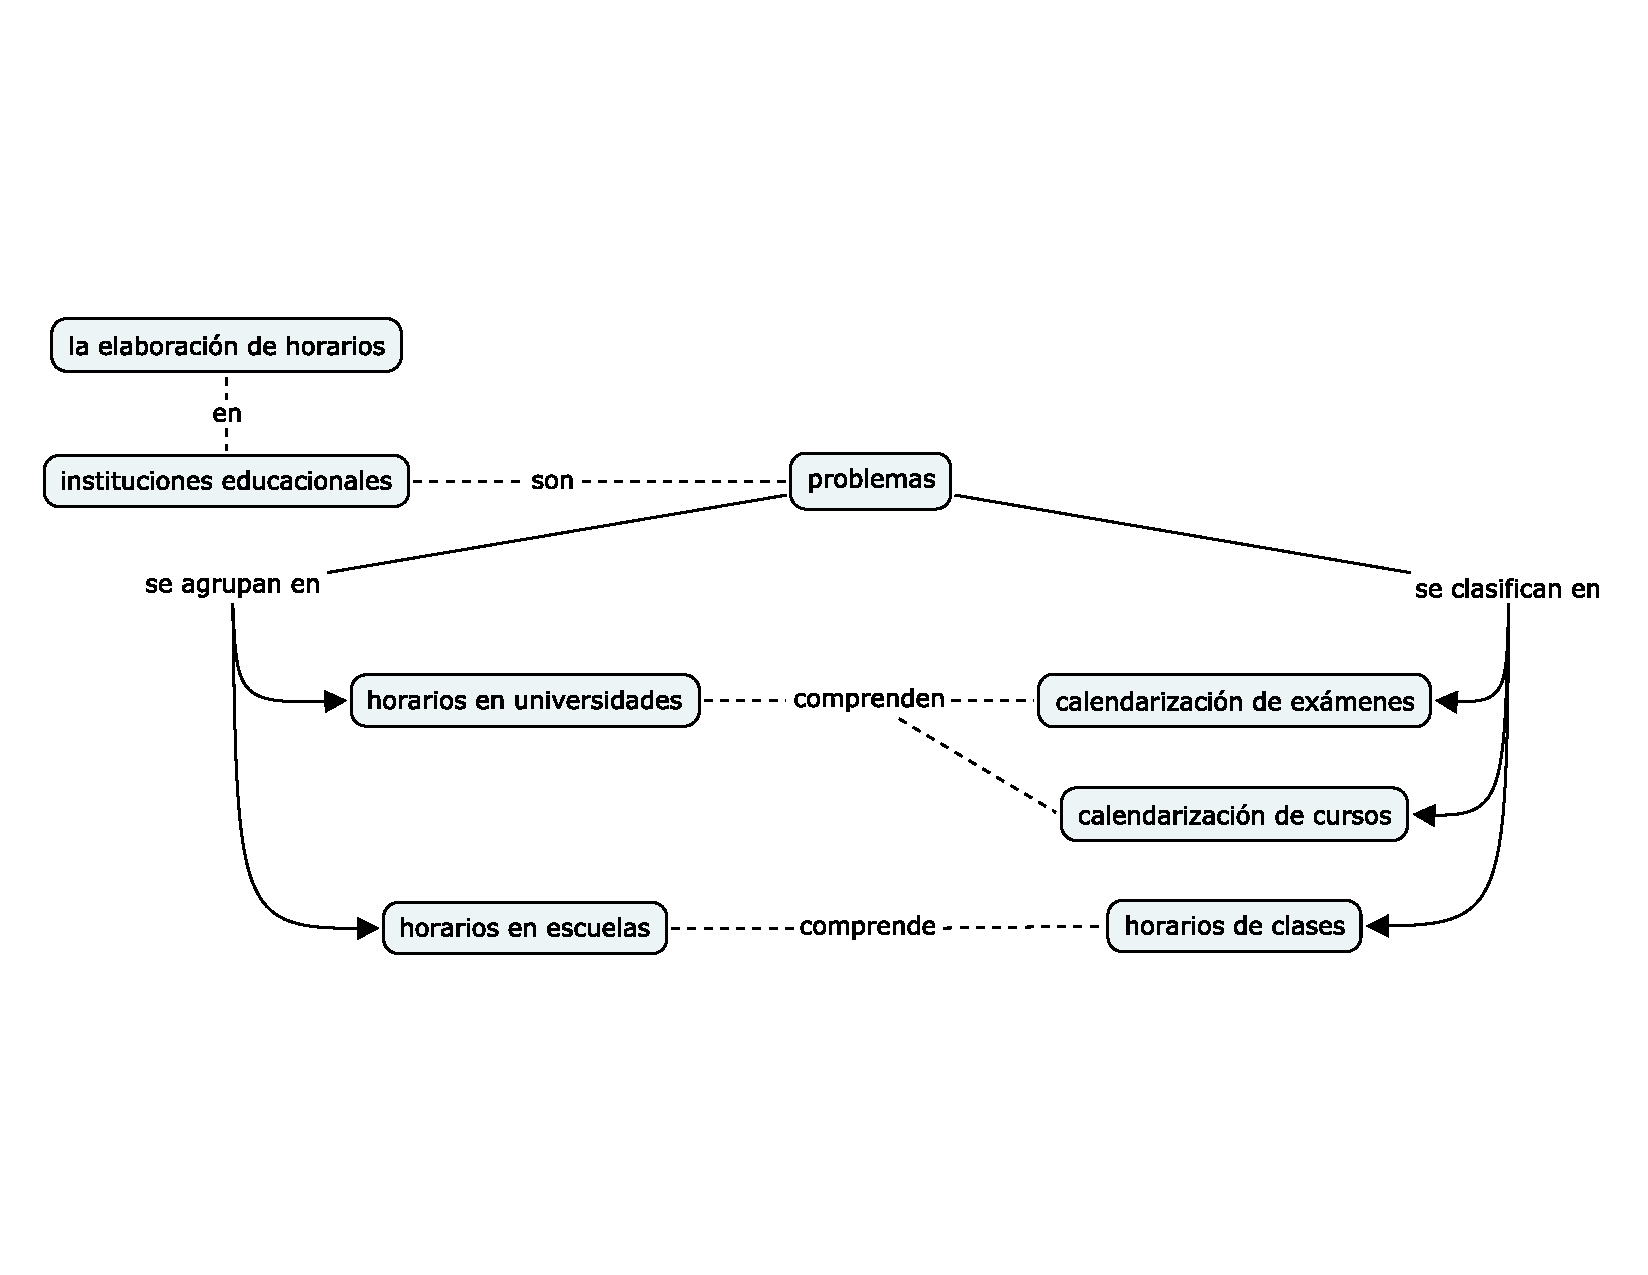
\includegraphics[width=.8\textwidth, trim=0 140 0 140]{timetabling_classification.pdf}
\caption[Clasificación del problema]{Clasificación de los problemas en la elaboración de horarios educacionales}
\label{fig:timetabling_classification}
\end{figure}

\subsection{Horarios en escuelas}

\index{horarios!en escuelas}

\subsubsection{Horarios de clases}

\index{horarios!de clases}
De acuerdo a \citet[p.~88]{schaerf99a-survey-of-automated} el problema de horarios de clases consiste en calendarizar en un periodo semanal todas las clases de una escuela, evitando que los profesores se encuentren con dos clases al mismo tiempo, y viceversa. \citet[p.~10,11]{abdullah06heuristic-approaches} elabora explicando que el problema consiste de un conjunto de profesores, clases, lecciones y periodos semanales. En donde tales periodos semanales son predefinidos.

El problema intenta asignar lecciones a periodos y, un profesor a una clase en particular en un momento dado mientras se satisface un conjunto de limitaciones con el fin producir un horario factible. Algunos ejemplos de limitaciones en este tipo de problemas son las capacidades de alojamiento, ubicaciones, cargas de trabajo de los profesores, tiempo de descanso entre lecciones.

\subsection{Horarios en universidades}

\index{horarios!en universidades}\index{calendarización!de cursos}\index{calendarización!de exámenes} 
El problema de la planificación de horarios en universidades puede ser agrupado en dos categorías: (i) calendarización de cursos y (ii) calendarización exámenes. 
El problema de la calendarización de cursos es el proceso de la asignación de periodos y aulas de manera tal que las reuniones entre conferenciantes y estudiantes pueda ocurrir. 
El problema de la calendarización de exámenes se refiere a la asignación de periodos y aulas de manera tal que los estudiantes puedan presentar sus exámenes. 
Ambos problemas son similares de manera superficial, pero existen diferencias importantes que los distinguen. 
En la calendarización de exámenes, múltiples exámenes pueden ser presentados en una misma aula (ej. auditorio) al mismo tiempo. 
Sin embargo, esto no es posible para la calendarización de cursos en donde únicamente un curso puede ser asignado a un aula \citep[p.~11]{abdullah06heuristic-approaches}.

\subsubsection{Calendarización de exámenes}

\index{calendarización!de exámenes}\index{calendarización!de cursos}
\citet[p.~4]{carter95recent-developments} definió el problema como la asignación de exámenes a un número limitado de periodos de manera tal que no existan conflictos o coincidencias. Los problemas de calendarización de cursos y exámenes son similares pero algunas diferencias relevantes según \citet[p.~159]{werra85an-introduction-to-timetabling} son:
\begin{enumerate}[a]
\item Existe generalmente un solo exámen por cada tema (mientras que hay varias exposiciones en un curso)
\item En la calendarización semanal de cursos, el objetivo principal es evitar conflictos (ej. la ocurrencia de que dos cursos elegidos por un mismo estudiante sean programados en el mismo periodo). Para los exámenes, generalmente se pide un máximo de un examen por día para cada estudiante o de ser posible, evitar la calendarización de exámenes en días consecutivos si el periodo de evaluación de exámenes lo permite.
\end{enumerate}
El problema de la calendarización de exámenes es muy común tanto en escuelas como en universidades. La asignación de los exámenes a los periodos está sujeta a un conjunto de limitaciones \citep[p.~12]{abdullah06heuristic-approaches}.

\subsubsection{Calendarización de cursos}

\index{calendarización!de cursos}
El problema de la calendarización de cursos surge cuando una universidad (o incluso una escuela) ofrece una colección de cursos (cada uno consistiendo de un número dado de conferencias) sin existir un currículo fijo y en donde cada estudiante puede elegir cierto número de cursos. El problema consiste en la asignación de cada lectura a algún periodo en la semana de manera tal que ningún estudiante requiera asistir a más de una conferencia a la vez \citep[p.~157]{werra85an-introduction-to-timetabling}. 
\citet[p.~88]{schaerf99a-survey-of-automated} define el problema como la calendarización semanal de todas las lecciones de un conjunto de cursos universitarios, minimizando los empalmes de las lecciones de cursos teniendo estudiantes en común.

\index{timetabling!university|see{planificación de horarios en universidades}}
\index{timetabling!school|see{horarios de clases y planificación de horarios en escuelas}}
\index{timetabling!course|see{calendarización de cursos}}
\index{timetabling!examination|see{calendarización de exámenes}}

\index{scheduling|see{planificación}}
\index{timetabling|see{planificación de horarios}}

% Bibliography
\bibliographystyle{apalike}
\bibliography{/Users/harciga/Dropbox/bibliographies/reviewed}
\bibliography{/Users/harciga/Dropbox/bibliographies/Dissertation books}
{
\RaggedRight
\printindex
}
\end{document}
